\documentclass[11pt]{article}

\usepackage[margin=1.05in]{geometry}
\usepackage{amsmath,amssymb,amsthm}
\usepackage{stmaryrd}
\usepackage{booktabs}
\usepackage{enumitem}
\usepackage{tikz}
\usepackage{listings}
\usepackage[expansion=false]{microtype}
\usepackage{hyperref}
\usepackage{palatino}
\usetikzlibrary{arrows.meta,positioning,decorations.pathmorphing,calc}

\hypersetup{colorlinks=true, linkcolor=blue!45!black,
            citecolor=blue!45!black, urlcolor=blue!45!black}

\theoremstyle{plain}
\newtheorem{theorem}{Theorem}[section]
\newtheorem{proposition}[theorem]{Proposition}
\newtheorem{lemma}[theorem]{Lemma}
\newtheorem{corollary}[theorem]{Corollary}
\newtheorem{conjecture}[theorem]{Conjecture}
\theoremstyle{definition}
\newtheorem{definition}[theorem]{Definition}
\newtheorem{observation}[theorem]{Observation}
\newtheorem{principle}[theorem]{Principle}
\theoremstyle{remark}
\newtheorem{remark}[theorem]{Remark}

\newcommand{\Tok}{\mathsf{T}}
\newcommand{\Sig}{\Sigma}
\newcommand{\Rpos}{\mathbb{R}_{>0}}
\newcommand{\Real}{\mathbb{R}}
\newcommand{\Reff}{R_{\mathrm{eff}}}
\newcommand{\bt}{\beta_1}
\newcommand{\Vt}{\mathsf{V}}
\newcommand{\Ct}{\mathsf{C}}
\newcommand{\Ot}{\mathsf{O}}
\newcommand{\Win}{\mathcal{W}}
\newcommand{\Cit}{\mathsf{Citizen}}
\newcommand{\quo}[1]{@#1}
\newcommand{\drop}[1]{*#1}

\lstset{
  basicstyle=\ttfamily\scriptsize,
  columns=fullflexible,
  breaklines=true,
  showstringspaces=false,
  commentstyle=\color{black!55},
  frame=single,
  framesep=4pt,
  xleftmargin=6pt,
  aboveskip=8pt,
  belowskip=8pt
}

\setlength{\emergencystretch}{2.5em}

\title{\bfseries Votes and Capital\\[0.35em]
\large Obstructions to conversion in a cost-accounted polity,
and the yield of the political cycle as the rule of law}
\author{L.G. Meredith\\ \small F1R3FLY.io}
\date{23 August 2026 --- working note}

\begin{document}
\maketitle

\begin{abstract}
Two token colours are put in one cost-accounted rho world: a franchise token
$\Vt$, issued one per registered citizen in a pre-election phase and spendable
only at a ballot, and a capital token $\Ct$, unequally held and spendable
everywhere else. Both are linear. The question is when a conversion path from
$\Ct$ to $\Vt$ collapses the distinction between what the polity may decide and
what money may buy. The answer offered here is that the pathology is not the
conversion edge but the \emph{cycle}: capital buys votes, votes buy an office,
the office pays rent, and the rule of law is the statement that this closed
path has yield at most one. That places the question inside the no-arbitrage
apparatus of \cite{vtok} and the cycle-space error-correction apparatus of
\cite{engine}, and both do real work. Four consequences are drawn out. First,
arbitrage removal is \emph{not} the repair: its fixed point is the polity in
which a vote is correctly priced at the office's rent per member of the quorum,
so the obstruction wanted here is the deletion of an edge, not the adjustment
of a rate. Second, the capture cost is a minimum-weight winning coalition, so
it is an order statistic of the lower tail of civic virtue and not a function
of its mean; with the mean held fixed at $100$, dispersion alone moves the
capture cost from $5100$ to $2076.58$ and flips the polity from safe to
captured. Third, the first Betti number of the conversion graph counts, with
one number, both the audit budget of the price code and the number of
independently purchasable offices. Fourth, typing the franchise
constitutively and demanding co-authentication at the ballot does obstruct the
\emph{sale} of a vote --- and converts it into a \emph{delegation} whose cycle
yield is larger by exactly the tenure $T$. Computations in \texttt{polity.py};
a three-citizen world in \texttt{polity.rho}.
\end{abstract}

\section{Introduction}

The preceding notes in this series asked how to \emph{remove} arbitrage
\cite{vtok,engine}. This one asks the opposite question. There are conversions
one wants to be impossible. A polity that distributes a franchise equally and
then permits it to be exchanged for capital has, in the usual phrase, sold the
rule of law; and the interesting formal question is what exactly has to be
absent from the world for that sale not to be available, and what the price of
its absence is.

The setting is cost-accounted rho \cite{CAR2026} with located token stacks
\cite{finrho,CGC2026}: a stack is a message on a channel, and the right to
spend from it is exactly the right to receive on that channel. Two colours are
in play. The franchise $\Vt$ is issued one per registered citizen in a
pre-election phase --- a proxy for checking the register --- and is accepted
only by the ballot. Capital $\Ct$ is held in whatever distribution capital is
held in and is accepted by the market. Both are linear: a token is consumed by
the receive that reads it, and no rule of the calculus copies one.

The thesis of the note is a single displayed quantity. Let $q$ be the quorum,
$\theta$ the price of a vote, $R$ the rent the office dispenses per epoch and
$T$ its tenure. Then
\[
  Y \;=\; \frac{RT}{q\theta}
\]
is the yield of the closed path
$\Ct \to \Vt^{\ast q} \to \Ot \to \Ct$, and the rule of law is the statement
$Y \le 1$. Everything else in the note is either a consequence of that
statement or an account of what the statement leaves out.

\subsection*{What is imported}

From \cite{vtok}: conversion systems over a signature monoid, the log-rate
cochain, arbitrage as non-unit cycle yield, and the equivalence between
arbitrage-freeness and the existence of a valuation. That paper works with
\emph{reversible} engines; \S\ref{sec:cycle} departs from it deliberately, and
\S\ref{sec:shown} records the departure.

From \cite{engine}: engines as edges, the detection theorem
$\lVert \text{syndrome}\rVert^2 = a^2\bigl(1-\Reff(e)\bigr)$, Foster's
identity $\sum_e (1-\Reff(e)) = \bt$ as the total detection budget of the price
code, ``bridges fail twice'', and the reading of interposition as the general
error model of a medium.

From \cite{quorum}: quorum structures as the opens of a semitopology, and the
observation that a coalition is as strong as its weakest member. Here the
inequality runs the other way: a polity is as corruptible as its cheapest
quorum.

From \cite{typedval}: the constitutive/possessive distinction, and the
mixed-zone (\textsc{dill}-style) calculus in which reputational hypotheses are
unrestricted and value hypotheses linear. \S\ref{sec:sale} is where that
distinction earns its keep.

From \cite{finrho}: located stacks, and the slogan that authority is possession
of a name and never adjacency. Everything in \S\ref{sec:sale} turns on it.

\subsection*{What is assumed away}

The ballot funds its own metering. In cost-accounted rho a rendezvous burns
phlogiston, so a ballot whose gate is paid by the voter has a poll tax built
into it and the effective franchise of citizen $i$ is
$\min\bigl(\Vt_i, \lfloor \sigma_i / \text{gate}\rfloor\bigr)$. That is a real
leak and a different note; here every ballot is free at the point of use.

\section{The polity}
\label{sec:polity}

\begin{definition}[The world]
Fix $n$ citizens $A_1,\dots,A_n$ and an epoch counter. The world is the
parallel composition of
\begin{enumerate}[label=(\roman*),leftmargin=2.2em]
\item a \emph{roll}, a persistent process answering whether a signature is
registered;
\item an \emph{issue} phase, which at the start of each epoch places one $\Vt$
token on the located stack $v_i = \quo{[\drop{\text{roll}}, e, \Sig(A_i)]}$ for
each registered $A_i$;
\item a \emph{ballot}, which consumes $\Vt$ tokens and, on reaching quorum $q$
for one choice, emits the \emph{office} capability;
\item a \emph{rent} engine, which pays $R$ units of $\Ct$ per epoch to the
holder of the office for $T$ epochs;
\item a \emph{market}, which consumes $\Ct$ and delivers goods and services.
\end{enumerate}
Appendix~\ref{app:rho} gives all five for $n=3$, $q=2$.
\end{definition}

Three points about the issue phase deserve emphasis, because the rest of the
note leans on them.

\begin{observation}[The franchise is a source, not a mint]
Nothing in the issue phase creates a token that was not already entailed by the
roll. In the access-profile classification of \cite[\S10]{scientist} the roll is
a \emph{source}: persistent, rate-limited, non-exclusive, non-adaptive --- and
here additionally \emph{keyed to identity}. Capital is \emph{stock}: exhaustible,
exclusive, accumulable. The whole of \S\ref{sec:ratchet} is a consequence of
this difference in profile rather than of any difference in quantity.
\end{observation}

\begin{observation}[Two zones, one token]
The roll is non-rivalrous: consulting it does not deplete it, and contraction
is sound on the hypothesis $\Gamma \vdash \Sig(A_i) : \Cit$. The issued token is
rivalrous: casting it consumes it. So the franchise is \emph{constitutive in
origin and possessive in circulation}, and the issue phase is precisely the
dereliction
\[
  \Gamma \vdash\; !\,\Cit(A_i) \quad\longmapsto\quad \Gamma\,;\,\Delta \vdash v_i : \Vt(A_i)
\]
metered to one dereliction per epoch. This is the mixed-zone calculus of
\cite[\S6.3]{typedval} with a rate limit attached to the dereliction rule.
\end{observation}

\begin{observation}[Locations are names]
Because $\mid$ is associative--commutative, a stack that floats in the soup is
adjacent to every process in it, which is ambient authority
\cite[\S2.2]{finrho}. Every stack here is held on a channel. The consequence
that matters is negative: the object of a bribe is not the token but the
\emph{channel}, and the calculus has no rule that prevents a process from
sending a name it holds.
\end{observation}

\section{The political cycle and its yield}
\label{sec:cycle}

\subsection{The conversion graph}

Following \cite[\S2]{vtok} we work over the signature monoid $(\Sig,\ast,())$
and take the token set $\Tok = \{\Ct, \Vt, \Ot_1,\dots,\Ot_m\}$, closed under
$\ast$ on the fragment it names, so that $\Vt^{\ast q}$ is the compound
signature of a quorum's worth of franchise.

\begin{definition}[The political engines]
\label{def:engines}
$\Gamma_{\mathrm{pol}}$ has three families of engine.
\begin{align*}
  \varepsilon_i &: \Vt^{\ast q} \to \Ot_i, & r(\varepsilon_i) &= 1
    &&\text{the ballot: $q$ votes make one tenure;}\\
  \rho_i &: \Ot_i \to \Ct, & r(\rho_i) &= R_i T_i
    &&\text{the rent: a tenure pays $R_iT_i$;}\\
  \beta &: \Ct \to \Vt, & r(\beta) &= 1/\theta
    &&\text{the bribe: $\theta$ capital buys one vote.}
\end{align*}
\end{definition}

\begin{remark}[Irreversibility, and why the vtok theorem must be restated]
\label{rem:irrev}
Definition~2.1 of \cite{vtok} imposes $r(a\to b)\,r(b\to a) = 1$, which makes
every engine an undirected edge. That is wrong here. An office cannot be
converted back into $q$ votes; a delivered service cannot be converted back into
capital. The political engines are one-way, and $\Gamma_{\mathrm{pol}}$ is a
\emph{directed} graph. The correct restatement is the standard
negative-cycle/potential duality, which specialises to \cite[Thm.~3.3]{vtok}
when every edge is present in both orientations.
\end{remark}

\begin{theorem}[Sub-valuations and directed cycles]
\label{thm:ftap}
Let $\Gamma$ be a finite directed conversion graph with rates
$r : E \to \Rpos$ and log-rates $\ell = \log r$. The following are equivalent.
\begin{enumerate}[label=\textup{(\roman*)},leftmargin=2.2em]
\item No directed cycle has yield $>1$.
\item There is a \emph{sub-valuation}: a function $\nu : \Tok \to \Rpos$ with
$\nu(a) \ge r(a\to b)\,\nu(b)$ for every engine $a \to b$; equivalently a
potential $p = \log\nu$ with $\ell(a\to b) \le p(a) - p(b)$.
\item The longest-path problem for $\ell$ on $\Gamma$ is well posed.
\end{enumerate}
Moreover $\nu$ may be taken to be a valuation in the sense of
\cite[Def.~3.2]{vtok} --- with equality throughout --- if and only if every
directed cycle has yield exactly $1$.
\end{theorem}

\begin{proof}
(i)$\Rightarrow$(ii): adjoin a source vertex with zero-weight edges to every
token and let $p(a)$ be the longest $\ell$-weight of a path from the source to
$a$, finite because no positive-weight cycle exists. Relaxation of the edge
$a\to b$ gives $p(b) \ge p(a) + \ell(a\to b)$, whence
$\ell(a\to b) \le p(a) - p(b)$ after the sign convention of
\cite[Def.~3.2]{vtok}. (ii)$\Rightarrow$(i): telescope $p$ around a cycle; the
inequalities sum to $\sum \ell \le 0$, i.e.\ yield $\le 1$.
(i)$\Leftrightarrow$(iii) is Bellman--Ford. The last clause is
\cite[Thm.~3.3]{vtok} with path-independence replacing path-domination.
\end{proof}

\begin{remark}
The reading of Theorem~\ref{thm:ftap}(ii) is exactly the reading one wants of a
polity: \emph{every available conversion is value non-increasing}. A society in
which no sequence of legitimate and illegitimate moves returns more than it
consumed is a society with a coherent price for everything, including a price
for things that are not for sale. That is a strong statement, and
Corollary~\ref{cor:price} says how strong.
\end{remark}

\subsection{The theorem}

\begin{definition}[Rule of law]
\label{def:rol}
The polity satisfies the \emph{rule of law} when every directed cycle of
$\Gamma_{\mathrm{pol}}$ passing through a ballot engine has yield at most one.
It is \emph{captured} when some such cycle has yield greater than one and some
holder's purse covers its cost.
\end{definition}

\begin{theorem}[The political cycle]
\label{thm:cycle}
In the minimal polity ($m = 1$, one bribe engine, homogeneous vote price
$\theta$) the unique directed cycle through the ballot is
$\gamma = \beta^{\ast q};\varepsilon;\rho$, with yield
\[
  Y(\gamma) \;=\; \frac{RT}{q\theta}.
\]
Hence the rule of law holds if and only if $q\theta \ge RT$, and the polity is
captured if and only if additionally some purse satisfies $W \ge q\theta$.
\end{theorem}

\begin{proof}
Monoidal compatibility \cite[Def.~2.2]{vtok} gives
$r(\Ct^{\ast q}\to\Vt^{\ast q}) = \theta^{-q}$. Composing along $\gamma$:
$q\theta$ units of $\Ct$ yield $q$ units of $\Vt$, yield one tenure of $\Ot$,
yield $RT$ units of $\Ct$. Uniqueness of the cycle is
$\bt(\Gamma_{\mathrm{pol}}) = 1$ at $m=1$
(Proposition~\ref{prop:betti}).
\end{proof}

Two separate conditions appear, and conflating them is the commonest error in
informal discussion of this subject.

\begin{corollary}[Liquidity and profitability are different]
Capture requires both $RT > q\theta$ (the cycle is profitable) and
$W \ge q\theta$ (somebody can front the cost). A polity of many modest fortunes
can be safe against a cycle of enormous yield, and a polity with one great
fortune can be safe against a cycle of yield just under one. Only the first is
a property of the constitution; the second is a property of the wealth
distribution, and it moves.
\end{corollary}

\begin{corollary}[The price of the franchise]
\label{cor:price}
The polity sits exactly on the boundary of Definition~\ref{def:rol} iff
$\theta = RT/q$, and in that case, and only in that case, a valuation exists
with
\[
  \frac{\nu(\Vt)}{\nu(\Ct)} \;=\; \frac{RT}{q}.
\]
Arbitrage-freeness of a polity is therefore not the absence of a price for a
vote. It is the assertion that a vote \emph{has} one, namely the office's
lifetime rent divided by the quorum.
\end{corollary}

At $R = 1200$, $T = 4$, $q = 51$ the break-even vote price is
$\theta^\ast = 94.1176$.

\begin{corollary}[Arbitrage removal is not the repair]
\label{cor:reflection}
The arbitrage-removal reflection of \cite[\S4]{vtok} adjusts rates until the
cyclic component of the log-rate cochain vanishes. Applied to
$\Gamma_{\mathrm{pol}}$ it raises $\theta$ to $RT/q$: its fixed point is the
polity in which vote-buying is break-even rather than the polity in which it is
absent. The obstruction sought in this note is therefore \emph{not in the image
of the reflection}. It is the deletion of the edge $\beta$ --- a change to the
topology of $\Gamma_{\mathrm{pol}}$, not to its rates.
\end{corollary}

\begin{principle}[Two obstructions, one of which is a price]
\label{prin:two}
A polity may obstruct the conversion in exactly two ways. \emph{Topologically},
by ensuring that no capability reaches the franchise namespace from a
$\Ct$-holding one, which deletes $\beta$ and disconnects $\Vt$ from $\Ct$;
\cite[\S10]{engine} then says there is no common valuation and the two colours
are incommensurable. \emph{Economically}, by ensuring $RT \le q\theta$. The
second inequality is symmetric in $RT$ and $\theta$, which is the note's most
useful normative remark: \emph{bounding what an office may dispense and raising
the price of civic virtue are the same intervention}, and only one of the two is
under the constitution's control.
\end{principle}

\begin{figure}[t]
\centering
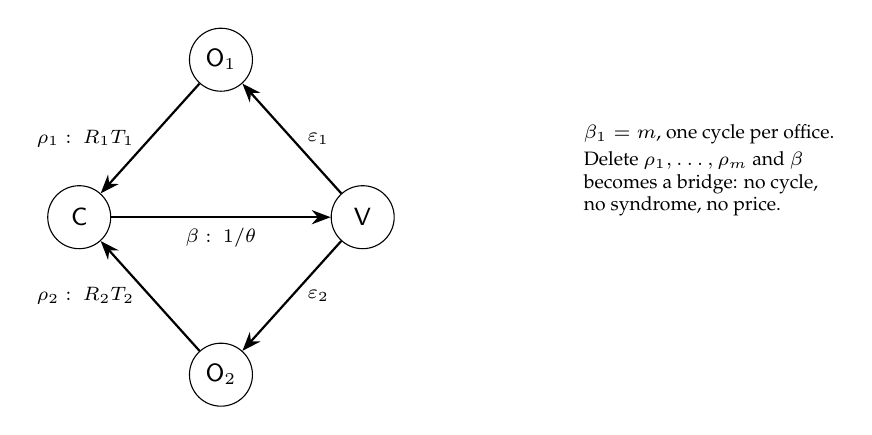
\begin{tikzpicture}[scale=1.0, every node/.style={font=\small},
  >={Stealth[length=2.4mm]}]
\node[circle,draw,minimum size=8mm] (C) at (0,0) {$\Ct$};
\node[circle,draw,minimum size=8mm] (V) at (3.6,0) {$\Vt$};
\node[circle,draw,minimum size=8mm] (O1) at (1.8,2.0) {$\Ot_1$};
\node[circle,draw,minimum size=8mm] (O2) at (1.8,-2.0) {$\Ot_2$};
\draw[->,thick] (C) -- node[below,font=\scriptsize]{$\beta:\ 1/\theta$} (V);
\draw[->,thick] (V) -- node[right,font=\scriptsize,xshift=2pt]{$\varepsilon_1$} (O1);
\draw[->,thick] (O1) -- node[left,font=\scriptsize,xshift=-2pt]{$\rho_1:\ R_1T_1$} (C);
\draw[->,thick] (V) -- node[right,font=\scriptsize,xshift=2pt]{$\varepsilon_2$} (O2);
\draw[->,thick] (O2) -- node[left,font=\scriptsize,xshift=-2pt]{$\rho_2:\ R_2T_2$} (C);
\node[align=left,font=\scriptsize] at (8.0,0.6)
  {$\bt = m$, one cycle per office.\\[2pt]
   Delete $\rho_1,\dots,\rho_m$ and $\beta$\\
   becomes a bridge: no cycle,\\
   no syndrome, no price.};
\end{tikzpicture}
\caption{The political conversion graph at $m=2$. Every cycle passes through
$\beta$; the first Betti number counts the offices.}
\label{fig:graph}
\end{figure}

\section{The capture cost is a minimum-weight winning coalition}
\label{sec:mincut}

Theorem~\ref{thm:cycle} assumed one price $\theta$ for every citizen. Dropping
that assumption is where the model starts to say something.

\begin{definition}[Quorum structure and capture cost]
A \emph{quorum structure} is an upward-closed family
$\Win \subseteq 2^{\{A_1,\dots,A_n\}}$ of winning coalitions --- in the language
of \cite{quorum}, a choice of opens. Given reservation prices
$\theta_1,\dots,\theta_n$, the \emph{capture cost} is
\[
  K(\Win,\theta) \;=\; \min_{S \in \Win} \sum_{i \in S} \theta_i .
\]
\end{definition}

\begin{proposition}[Order statistics]
\label{prop:order}
For the anonymous rule $\Win = \{S : |S| \ge q\}$, $K$ is the sum of the $q$
smallest reservation prices. It is therefore a functional of the \emph{lower
tail} of the distribution of civic virtue and not of its mean.
\end{proposition}

The consequence is sharp enough to be worth measuring. With $n = 101$,
$q = 51$, and reservation prices lognormal with the mean pinned at $100$:

\begin{center}
\begin{tabular}{lrrl}
\toprule
distribution & $K$ & $Y = RT/K$ & verdict\\
\midrule
every citizen prices at $100$ & $5100.00$ & $0.941176$ & rule of law holds\\
lognormal, mean $100$, $\sigma = 0.8$ & $2076.58$ & $2.311494$ & captured\\
\bottomrule
\end{tabular}
\end{center}

\begin{corollary}[The incorruptible are irrelevant]
\label{cor:irrelevant}
In the measured draw the $50$ dearest citizens hold $76.1\%$ of the aggregate
reservation price of the electorate and contribute nothing whatever to $K$.
Virtue concentrated above the $q$-th order statistic buys the polity no
protection at all.
\end{corollary}

This is the mirror image of the quorum algebra of \cite[\S6]{quorum}, where a
coalition is as strong as its weakest member because $\otimes$ is $\min$. Here
the polity is as corruptible as its cheapest quorum, and for the same reason:
the relevant operation over coalitions is a minimum, and a minimum is blind to
everything but its argmin.

\begin{table}[t]
\centering
\begin{tabular}{rrrl}
\toprule
$\sigma$ & $K$ & $Y = RT/K$ & \\
\midrule
$0.0$ & $5100.00$ & $0.941176$ & rule of law holds\\
$0.1$ & $4674.95$ & $1.026749$ & captured\\
$0.2$ & $4255.19$ & $1.128034$ & captured\\
$0.4$ & $3449.94$ & $1.391328$ & captured\\
$0.8$ & $2073.11$ & $2.315363$ & captured\\
$1.2$ & $1098.62$ & $4.369130$ & captured\\
$1.6$ & $\phantom{0}510.07$ & $9.410449$ & captured\\
\bottomrule
\end{tabular}
\caption{Common random numbers; the mean reservation price is held at $100.00$
throughout. The crossing $Y = 1$ occurs at $\sigma \approx 0.0687$. The sweep
uses its own standard-normal draw, held fixed across rows so that the curve is
monotone, so the $\sigma = 0.8$ row differs slightly from the independently
drawn $K = 2076.58$ of \S\ref{sec:mincut}.}
\label{tab:sigma}
\end{table}

\begin{proposition}[Dispersion alone captures the polity]
\label{prop:sigma}
Holding the mean reservation price fixed, the capture cost is strictly
decreasing in dispersion, and in the measured sweep
(Table~\ref{tab:sigma}) the yield crosses one at $\sigma \approx 0.0687$ ---
a coefficient of variation under $7\%$. The polity is not captured because
virtue is cheap on average. It is captured because virtue is
\emph{unevenly priced}.
\end{proposition}

\subsection{Districting}

\begin{proposition}[Nesting the rule lowers the cost twice]
\label{prop:district}
Replace the anonymous rule by a two-tier rule: $11$ districts of sizes
$10,10,9,\dots,9$ summing to $101$, a district won by an internal majority, the
office won by $6$ districts. Then
\begin{enumerate}[label=(\alph*),leftmargin=2.2em]
\item the minimal winning coalition shrinks from $51$ to $30$ citizens, which
lowers $K$ even at constant prices; and
\item the choice of \emph{which} citizens share a district is a free parameter
of the constitution, and choosing it adversarially lowers $K$ again.
\end{enumerate}
Measured: $K = 2076.58$ under the popular majority; $1205.40$ under a random
assignment of citizens to districts; $936.30$ under a packed assignment that
puts a bare majority of the cheapest citizens into each of six districts and
pads them with the dearest. The packed figure is $45.09\%$ of the
popular-majority price and requires the consent of $30$ of $101$ citizens,
$29.70\%$ of the electorate.
\end{proposition}

In the semitopological language of \cite{quorum} this is the observation that
$\Win$ is a \emph{choice of opens} and that the choice is priced. Gerrymandering
is not an abuse of a quorum structure; it is a move within the space of quorum
structures, and the model says exactly what the move is worth.

\begin{remark}[Raising the quorum is not free either]
$K$ is increasing in $q$, so unanimity maximises the capture cost among
anonymous rules --- and destroys liveness, since one holdout blocks every
outcome. This is the safety/liveness trade of \cite[\S11]{quorum} in its
constitutional dress, and it is why the interesting designs sit strictly between
$q = \lceil (n+1)/2\rceil$ and $q = n$.
\end{remark}

\section{The purchasable set}
\label{sec:purchasable}

The stated target was the condition under which \emph{all} collectively enabled
outcomes become purchasable. Two regimes appear, and the difference between
them is instructive.

\begin{proposition}[Anonymity forbids partial capture]
\label{prop:phase}
If all reservation prices are equal and the quorum structure is anonymous, then
every collectively enabled outcome has the same capture cost $K$. The
purchasable set is therefore empty for $W < K$ and the whole of the
collectively enabled set for $W \ge K$: there is no purse that buys some
outcomes and not others.
\end{proposition}

\begin{corollary}
Equality of the franchise, which is what makes the polity fair, is also what
makes its corruption a phase transition rather than a gradient. A model with
graded capture must get the grading from somewhere other than the distribution
of votes.
\end{corollary}

It gets it from prior alignment. Give each outcome $\varphi$ a set of natural
supporters $S(\varphi)$; then the briber need only buy $q - |S(\varphi)|$
opponents, and cheapest-first:
\[
  K(\varphi) \;=\; \textstyle\sum \bigl\{\text{the } q - |S(\varphi)| \text{ smallest }
  \theta_i \ :\ i \notin S(\varphi)\bigr\},
\]
with $K(\varphi) = 0$ when $|S(\varphi)| \ge q$.

\begin{table}[t]
\centering
\begin{tabular}{rr}
\toprule
purse $W$ & purchasable share\\
\midrule
$0$ & $50.00\%$\\
$250$ & $63.60\%$\\
$500$ & $73.50\%$\\
$1000$ & $89.45\%$\\
$1500$ & $99.75\%$\\
$2000$ & $100.00\%$\\
\bottomrule
\end{tabular}
\caption{$2000$ outcomes, alignment drawn per outcome; heterogeneous
reservation prices as in \S\ref{sec:mincut}. Half the outcomes command a
natural majority and are free.}
\label{tab:purse}
\end{table}

\begin{proposition}[The price of everything]
\label{prop:everything}
In the measured world a purse of $W^\ast = 1663.38$ purchases \emph{every}
collectively enabled outcome. That is $80.10\%$ of the price of a bare quorum
and $34.65\%$ of a single tenure's rent.
\end{proposition}

The last figure is the one to hold on to. The purse that buys the entire
legislative output of the polity is a third of what the office pays out in one
tenure. The reason is Corollary~\ref{cor:irrelevant} acting twice: an outcome
with any natural support needs fewer than $q$ purchases, and the purchases it
needs are the cheapest available.

\section{Detection}
\label{sec:detect}

\begin{proposition}[The Betti number counts the offices]
\label{prop:betti}
For $\Gamma_{\mathrm{pol}}$ with $m$ rent-bearing offices sharing one bribe
edge, $|V| = m+2$, $|E| = 2m+1$ and $\bt = |E| - |V| + 1 = m$.
\end{proposition}

\begin{theorem}[Foster, imported {\cite[Thm.~5.4]{engine}}]
\label{thm:foster}
$\sum_{e} \bigl(1 - \Reff(e)\bigr) = \bt$: the total detection strength of the
price code is the first Betti number, distributed among the edges by geometry.
\end{theorem}

Verified numerically for $m = 1,\dots,6$ in \texttt{polity.py}: the sum equals
$m$ to six decimal places in every case.

\begin{proposition}[The strength of the bribe edge]
\label{prop:bribe}
In $\Gamma_{\mathrm{pol}}$ with unit edge weights,
$1 - \Reff(\beta) = m/(m+2)$: it is $1/3$ at one office, $1/2$ at two,
$3/5$ at three and $3/4$ at six.
\end{proposition}

\begin{proof}
The $m$ office paths from $\Vt$ to $\Ct$ each have resistance $2$ and are in
parallel, giving $2/m$; that is in parallel with the unit edge $\beta$, giving
$\Reff(\beta) = 2/(m+2)$.
\end{proof}

\begin{corollary}[The lone drain is invisible]
\label{cor:drain}
If the office bears no rent --- delete every $\rho_i$ --- then $\beta$ lies on
no cycle. By \cite[Thm.~5.3]{engine} its syndrome is identically zero, and by
\cite[Cor.~5.6]{engine} its rate is unconstrained by no-arbitrage: any price for
a vote extends to a consistent sub-valuation. In a polity with nothing to sell,
the price of a vote is both undetectable and undetermined; a citizen may sell
the franchise for a drink and no audit will register it, because there is
nothing for the audit to be inconsistent \emph{with}.
\end{corollary}

\begin{principle}[Separation of powers is a first Betti number]
\label{prin:powers}
The audit budget of the price code over $\Gamma_{\mathrm{pol}}$ is exactly the
number of independently rent-bearing offices.
\end{principle}

That is the pleasant half. The unpleasant half is that the same number counts
something else.

\begin{proposition}[$\bt$ is two-edged]
\label{prop:twoedged}
$\bt = m$ counts, simultaneously, the audit budget of
Theorem~\ref{thm:foster} and the number of independently purchasable offices.
Adding an office adds a cycle, and a cycle is both a check and an opportunity.
\end{proposition}

The obvious repair --- divide one office of rent $RT$ into $m$ offices of rent
$RT/m$ --- does less than one hopes.

\begin{proposition}[Division of the office]
\label{prop:division}
If the $m$ divided offices are elected by the \emph{same} electorate, one
purchased quorum wins all of them at once, the capture cost is unchanged, and
the aggregate yield is unchanged at $RT/K$: division buys audit budget and
nothing else. If they are elected by \emph{disjoint} blocks, the cost of total
capture rises --- measured $2076.58 \to 2267.96 \to 2402.77 \to 2691.25$ for
$m = 1,3,5,11$ --- because the briber may no longer cherry-pick globally; but
the yield of the \emph{cheapest single office} does not fall, measured
$2.311494, 2.470722, 2.361207, 2.332065$. Partial capture remains exactly as
profitable as total capture was.
\end{proposition}

\begin{remark}[A labelled negative result]
Proposition~\ref{prop:division} is stated as a negative result and kept. The
tidy story --- separate the powers and the yield divides --- is false in this
model, and the reason is structural rather than numerical: the yield of a cycle
is a ratio, and dividing the rent divides the numerator and the number of
purchases equally.
\end{remark}

\begin{remark}[The honest caveat about detection]
\label{rem:transparency}
Theorem~\ref{thm:foster} prices \emph{rate faults on observable edges}. The
bribe edge is the least observable edge in the graph: reading it requires
grade-one access to a private rendezvous, which in the classification of
\cite[\S2]{scientist} is exactly what an outsider does not have. So the realised
detection strength is $\bt$ scaled by transparency, and a constitution that
multiplies offices while leaving $\beta$ unobservable has bought a budget it
cannot spend. \S\ref{sec:sale} approaches this from the other side and finds one
mechanism that makes the corrupt edge visible --- at a price.
\end{remark}

\section{The ratchet}
\label{sec:ratchet}

\begin{proposition}[A stock cannot be outbid by a flow]
\label{prop:ratchet}
The franchise is re-issued each epoch and is not accumulable: an unspent $\Vt$
token is void at the next registration. Capital persists. Hence a defensive
counter-bid --- citizens outbidding a briber for their own votes --- must be
funded from stock, and the electorate's stock is the thing capital exists to
spend, while the incumbent's stock is fed by $\rho$.
\end{proposition}

Measured, with $K = 2076.58$, $RT = 4800$, net $2723.42$ per tenure, against an
electorate whose combined capital stock is $49{,}108.98$: the incumbent's stock
passes the whole electorate's at tenure $18$, that is after $72$ epochs, over
which $7272$ votes were issued and none of them stored.

\begin{corollary}
The asymmetry that drives capture is between \emph{access profiles} --- source
against stock --- and not between quantities. Equalising the initial
distribution of capital would delay the crossing; it would not change its
direction, because only one side of the exchange compounds.
\end{corollary}

\section{Sale, delegation, and the price of co-authentication}
\label{sec:sale}

The remaining question is whether typing the franchise correctly obstructs the
edge $\beta$ at all. The answer is a qualified yes with an unwelcome
quantitative tail.

\begin{proposition}[Anonymity of send; constitutive typing alone obstructs nothing]
\label{prop:anon}
A rho send carries no sender. A ballot whose guard consumes the token
$\Vt(A_i)$ and inspects its content therefore cannot distinguish a cast by
$A_i$ from a cast by any process holding the located stack channel $v_i$.
Consequently the constitutive \emph{typing} of the franchise --- the fact that
the token records whose franchise it is --- obstructs nothing on its own: a
briber holding $q$ distinct tokens casts $q$ distinct identities and the ballot
is satisfied.
\end{proposition}

\begin{definition}[Co-authenticating ballot]
The \emph{co-authenticating} ballot's guard demands two things: the linear token
$\Vt(A_i)$, and a \emph{fresh attestation} obtained by drawing on the roll at
cast time, i.e.\ a witness for $\Gamma \vdash \Sig(A_i) : \Cit$ produced during
this ballot.
\end{definition}

\begin{theorem}[Sale collapses to delegation]
\label{thm:collapse}
Under the co-authenticating ballot, no transfer of linear tokens enables a cast.
To cast on behalf of $A_i$ a briber must obtain a capability that draws on the
roll. Because the roll is unrestricted, that capability is not consumed by use:
it is a \emph{standing delegation}, persistent in the term as an interposed
forwarder on the path to $v_i$.
\end{theorem}

\begin{proof}
The guard is satisfiable only by a message produced by the attestation contract,
which consults the roll. The roll answers on the signature, and the signature is
not a transferable resource in $\Delta$ but a subject position in $\Gamma$; so
the briber's only route is to hold a name whose receipt triggers the
attestation. Holding such a name is possession of a capability drawing on an
unrestricted hypothesis, on which contraction is admissible; hence it survives
use.
\end{proof}

\begin{corollary}[Visibility]
A sale leaves nothing behind: the token is consumed and the ballot's transcript
is identical to an honest one. A delegation leaves a persistent forwarder, which
is an interposed medium in the sense of \cite[\S5]{engine} and therefore a
spatial-behavioural formula an auditor can look for. Co-authentication buys the
observability that Remark~\ref{rem:transparency} said the audit budget needed.
\end{corollary}

\begin{theorem}[The price of visibility]
\label{thm:price-vis}
Because $\Vt$ is re-issued at every registration, a sale must be repurchased
every epoch, costing $TK$ over a tenure; a delegation is bought once per tenure,
costing $K$. Hence
\[
  Y_{\mathrm{del}} \;=\; T\cdot Y_{\mathrm{sale}} .
\]
\end{theorem}

Measured at $T = 4$: the sale arrangement costs $8306.32$ per tenure and yields
$0.577873$ --- the polity is safe. The delegation arrangement costs $2076.58$
and yields $2.311494$ --- the polity is captured. The ratio of yields is
$4.000000$, exactly the tenure. The delegation cycle becomes profitable as soon
as $T > K/R = 1.7305$.

\begin{principle}[Co-authentication trades expense for visibility]
\label{prin:trade}
Demanding co-authentication at the ballot converts an invisible, expensive
corruption into a visible, cheap one, with the discount factor equal to the
tenure. Whether that is a good trade depends entirely on whether anyone is
looking; and Remark~\ref{rem:transparency} shows that ``anyone looking'' is
itself a budgeted quantity.
\end{principle}

\begin{remark}[This is what one observes]
The corrupt relationships that survive in polities with authenticated ballots
are exactly the durable, visible, cheap ones: party machines, whipped blocs,
custodial staking, delegated proof of stake. The framework predicts that shape
from the metering discipline alone --- the linear zone is re-issued per epoch,
the unrestricted zone is not --- and does not need a story about human motives
to do it.
\end{remark}

\section{What is shown and what is not}
\label{sec:shown}

\paragraph{Shown.} That the pathology is a cycle and not an edge
(Theorem~\ref{thm:cycle}); that arbitrage removal prices the franchise instead
of protecting it (Corollary~\ref{cor:reflection}); that the capture cost is an
order statistic of the lower tail and that dispersion alone flips the verdict
(Propositions~\ref{prop:order}, \ref{prop:sigma}); that anonymity makes capture
a phase transition and alignment supplies the gradient
(Proposition~\ref{prop:phase}, Table~\ref{tab:purse}); that $\bt$ counts audit
budget and purchasable offices with one number
(Propositions~\ref{prop:betti}--\ref{prop:twoedged}); and that
co-authentication converts sale into delegation at a yield multiple of $T$
(Theorems~\ref{thm:collapse}, \ref{thm:price-vis}).

\paragraph{Not shown.}
\begin{itemize}[leftmargin=1.4em]
\item \emph{The reservation prices are exogenous.} A citizen's $\theta_i$ ought
to depend on what the office will do with the purchased outcome, which makes
$\theta$ a function of $K$ and the whole system a fixed point. Nothing here
solves that fixed point.
\item \emph{Coercion is not distinguished from sale.} Both appear in the model
as a transfer at price $\theta_i$; a coerced transfer has $\theta_i$ negative in
the citizen's own accounting, which the present bookkeeping cannot represent.
\item \emph{The secret ballot is deliberately absent.} With the hidden-name
quantifier retired \cite[\S3]{scientist}, concealment in this framework is a
price and never a wall, so a secret ballot would enter as an \emph{expense on
the buyer's assay} --- the buyer cannot verify delivery, so the purchased good
is observable only at a budget-relative $\bot$. That is the natural next note
and it is not attempted here.
\item \emph{Reversibility was dropped by hand.} Remark~\ref{rem:irrev} restates
\cite[Thm.~3.3]{vtok} for directed graphs; the restatement is standard, but the
Hodge decomposition of \cite[\S4]{vtok} does not transport to the directed
setting without work, and Corollary~\ref{cor:reflection} therefore appeals to
the reflection in its reversible form.
\item \emph{No dynamics.} Everything is per-epoch bookkeeping. Running the
polity under the Gillespie discipline of \cite{weighted} would let the ratchet
of \S\ref{sec:ratchet} be a rate rather than a recurrence.
\end{itemize}

\section{Open problems}

\begin{enumerate}[leftmargin=1.8em]
\item \textbf{Endogenous virtue.} Solve the fixed point
$\theta = \Theta(K(\theta))$. Does it have a stable solution, and is the stable
one above or below $RT/q$?
\item \textbf{A coreflection for edge deletion.} Arbitrage removal is an
idempotent reflection on rates. Is there a companion operation on
\emph{topology} --- deletion of the minimal set of edges disconnecting two
colours --- and is it a coreflection? Principle~\ref{prin:two} says the two
obstructions are different in kind; a categorical statement of the difference
would be worth having.
\item \textbf{The secret ballot as an engineered $\bot$.} Formalise
unverifiability of delivery as a budget-relative bottom in the assay trichotomy
of \cite[\S4]{scientist}, and compute what it does to $Y$.
\item \textbf{Three colours.} Add reputation as a third, non-transferable
colour and ask which conversions among $\{\Vt,\Ct,\text{Rep}\}$ must be absent.
\cite{typedval} suggests the interesting edges are the ones into and out of the
unrestricted zone.
\item \textbf{Learning the quorum structure.} \cite{quorum} makes the
semitopology the thing an observer is guessing. Here $\Win$ is given by the
constitution --- but a briber must \emph{discover} which coalitions are cheap,
and that search is itself priced. What does the ladder look like?
\item \textbf{Does the ratchet have a critical rent?} Below what $R$ does the
incumbent's stock fail to compound faster than the electorate's spends down?
\end{enumerate}

\appendix

\section{The three-citizen world}
\label{app:rho}

\texttt{polity.rho} gives the five components of \S\ref{sec:polity} for $n = 3$,
$q = 2$, together with the forbidden exchange contract (commented out, since its
presence is the thing under study) and the co-authenticating ballot with one
delegation. Three details are worth pointing at.

\paragraph{A.1 Located franchise.} The issue phase writes to
$v_i = \quo{[\drop{\text{roll}}, e, \Sig(A_i)]}$. The name is manufactured by
quotation and is fresh in the sense of \cite[\S3]{scientist} --- no
\texttt{new} binder is needed, and none is used.

\paragraph{A.2 The guard is a ballot, not a market.} The guard
\texttt{where tok == (colour, voter, e) and colour == "V"} is what makes the
contract a ballot: it accepts one colour and rejects the other. There is no
sender to check, which is Proposition~\ref{prop:anon} in one line of code.

\paragraph{A.3 The forbidden edge is a capability transfer.} The commented
\texttt{exchange} contract does not move a token. It moves the right to receive
on $v_i$. Nothing in rho forbids sending a name one holds, which is why
Principle~\ref{prin:two}'s topological obstruction is a statement about who was
ever handed what, and not a rule of the calculus.

\section{The computations}
\label{app:computations}

\texttt{polity.py} is standard library only, seeded at $20260823$, and prints
every number quoted above to \texttt{polity-output.txt}. Sections \textsc{m1}
through \textsc{m9} correspond to \S\ref{sec:detect}, \S\ref{sec:cycle},
\S\ref{sec:mincut} (three sections), \S\ref{sec:purchasable},
\S\ref{sec:ratchet}, \S\ref{sec:sale} and
Proposition~\ref{prop:division} respectively. Effective resistances are computed
by grounding one vertex of the graph Laplacian and solving by Gaussian
elimination with partial pivoting; Foster's identity is then a check on the
implementation as well as a result, and it holds to six decimal places for
$m = 1,\dots,6$.

Parameters throughout: $n = 101$, $q = 51$, $R = 1200$ per epoch, $T = 4$
epochs, $RT = 4800$, mean reservation price $100$, $\sigma = 0.8$ unless a
sweep says otherwise.

\begin{thebibliography}{99}

\bibitem{CAR2026} L.G. Meredith et al.
\newblock \emph{Cost-accounted rho calculus}. F1R3FLY.io research notes, 2026.

\bibitem{CGC2026} L.G. Meredith et al.
\newblock \emph{Cost accounting as a monad on continued interactive GSLTs},
v2. F1R3FLY.io research notes, 2026. \S10.4, located resource stacks.

\bibitem{finrho} F1R3FLY.io.
\newblock \emph{Financial contract combinators in rholang}. 2026.
\S2.2, located token stacks: a correction.

\bibitem{vtok} F1R3FLY.io.
\newblock \emph{Energy as a virtual token}. Working note, July 2026.

\bibitem{engine} F1R3FLY.io.
\newblock \emph{Engines and individuals: token conversion between composed
learners, the cycle space as a price code, and error correction as the criterion
of individuation}. Working note, August 2026.

\bibitem{compose} F1R3FLY.io.
\newblock \emph{Composing learners}. Working note, August 2026.

\bibitem{scientist} F1R3FLY.io.
\newblock \emph{The mortal scientist: learning as cost-accounted computation in
a reflective higher-order calculus}. Working note, 2026.

\bibitem{quorum} F1R3FLY.io.
\newblock \emph{Quorum as a where-clause: coalition logic as a graded hypothesis
language for populations of computations}. Working note, August 2026.

\bibitem{typedval} F1R3FLY.io.
\newblock \emph{Typed value}. Position paper, 2026.

\bibitem{weighted} F1R3FLY.io.
\newblock \emph{Weighted GSLTs}, v2. Working note, 2026.

\bibitem{Miller2006} M.S. Miller.
\newblock \emph{Robust composition: towards a unified approach to access control
and concurrency control}. PhD thesis, Johns Hopkins University, 2006.

\bibitem{Benton1994} P.N. Benton.
\newblock A mixed linear and non-linear logic: proofs, terms and models.
\newblock \emph{CSL}, 1994.

\bibitem{Girard1987} J.-Y. Girard.
\newblock Linear logic. \emph{Theoretical Computer Science} 50(1), 1987.

\bibitem{Foster1949} R.M. Foster.
\newblock The average impedance of an electrical network.
\newblock In \emph{Contributions to Applied Mechanics}, 1949.

\bibitem{KleinRandic} D.J. Klein and M. Randi\'c.
\newblock Resistance distance. \emph{Journal of Mathematical Chemistry} 12,
1993.

\bibitem{Bellman1958} R. Bellman.
\newblock On a routing problem. \emph{Quarterly of Applied Mathematics} 16,
1958.

\bibitem{HK} J.M. Harrison and D.M. Kreps.
\newblock Martingales and arbitrage in multiperiod securities markets.
\newblock \emph{Journal of Economic Theory} 20, 1979.

\bibitem{Tullock1967} G. Tullock.
\newblock The welfare costs of tariffs, monopolies, and theft.
\newblock \emph{Western Economic Journal} 5, 1967.

\bibitem{Krueger1974} A.O. Krueger.
\newblock The political economy of the rent-seeking society.
\newblock \emph{American Economic Review} 64(3), 1974.

\bibitem{Shapley1954} L.S. Shapley and M. Shubik.
\newblock A method for evaluating the distribution of power in a committee
system. \emph{American Political Science Review} 48(3), 1954.

\end{thebibliography}

\end{document}
